% ============================================================
%  Mapping Evaluation Frameworks for Language Learning Platforms
%  in Higher Education: A Scoping Review of Assessment Dimensions
%  and Coverage Gaps
%
%  IEEE Conference Format — IEEEtran
%  Draft v0.1 — May 2026
% ============================================================
\documentclass[conference]{IEEEtran}
\IEEEoverridecommandlockouts

% ── Encoding & fonts ─────────────────────────────────────────
\usepackage[T1]{fontenc}
\usepackage[utf8]{inputenc}
\usepackage{microtype}

% ── Mathematics ──────────────────────────────────────────────
\usepackage{amsmath,amssymb}

% ── Graphics ─────────────────────────────────────────────────
\usepackage{graphicx}
\graphicspath{{../../../images/}}   % relative path to images/ folder

% ── Tables ───────────────────────────────────────────────────
\usepackage{booktabs}
\usepackage{multirow}
\usepackage{array}
\usepackage{tabularx}
\usepackage{makecell}
\usepackage{rotating}

% ── Colours ──────────────────────────────────────────────────
\usepackage{xcolor}
\definecolor{fullcol}{HTML}{2e7d32}
\definecolor{partcol}{HTML}{f57f17}
\definecolor{nonecol}{HTML}{c62828}

% ── URLs & hyperlinks ─────────────────────────────────────────
\usepackage{url}

% ── Citations ────────────────────────────────────────────────
\usepackage{cite}

% ── Coverage symbols ─────────────────────────────────────────
\newcommand{\fullcov}{\textcolor{fullcol}{\textbf{\checkmark}}}
\newcommand{\partcov}{\textcolor{partcol}{\textbf{$\circ$}}}
\newcommand{\nocov}{\textcolor{nonecol}{\textbf{$\times$}}}

% ── Column types ─────────────────────────────────────────────
\newcolumntype{C}[1]{>{\centering\arraybackslash}p{#1}}
\newcolumntype{L}[1]{>{\raggedright\arraybackslash}p{#1}}

% ============================================================
\begin{document}

\title{Mapping Evaluation Frameworks for Language Learning
       Platforms in Higher Education: A Scoping Review of
       Assessment Dimensions and Coverage Gaps}

\author{%
  \IEEEauthorblockN{[Author 1 Name], [Author 2 Name]}
  \IEEEauthorblockA{%
    \textit{[Department, Faculty]}\\
    [Institution Name], [City, Country]\\
    \{author1, author2\}@institution.ac.id}
}

\maketitle

% ============================================================
\begin{abstract}
The proliferation of digital language learning platforms in higher
education has not been matched by evaluation frameworks capable of
assessing them comprehensively. Existing frameworks originate from
disparate disciplines, including Computer-Assisted Language Learning
(CALL), Information Systems (IS), and instructional design; each
provides only partial coverage of dimensions relevant to platform
quality. No single framework simultaneously addresses technology
architecture, pedagogical effectiveness, institutional governance,
and high-stakes testing specificity. This scoping review
systematically maps evaluation frameworks for digital language
learning and EdTech platforms in higher education, covering
literature published between 2001 and 2025. Following the five-stage
methodology of Arksey and O'Malley~\cite{b6} and reported in
accordance with PRISMA-ScR~\cite{b11}, this study identifies
12~preliminary frameworks and evaluates them against five object-level
evaluation dimensions derived from IS quality theory and language
assessment theory, supplemented by a separate framework rigor
indicator. A dimensional coverage matrix shows that no existing
framework exceeds a coverage score of~2.5/5.0, and the high-stakes
test specificity dimension achieves at most partial coverage across
all reviewed frameworks. These results confirm systematic disciplinary
fragmentation and provide an empirical baseline for developing an
integrated evaluation framework.
\end{abstract}

\begin{IEEEkeywords}
CALL evaluation; EdTech assessment framework; scoping review;
dimensional gap analysis; higher education
\end{IEEEkeywords}


% ============================================================
\section{Introduction}
\label{sec:intro}
% ============================================================

The expansion of Computer-Assisted Language Learning (CALL),
Mobile-Assisted Language Learning (MALL), and language test
preparation platforms within higher education ecosystems has created
an urgent need for systematic and reproducible evaluation mechanisms.
Institutions now face complex adoption decisions, selecting,
retaining, or discontinuing EdTech platforms on evidence that is
academically and managerially defensible~\cite{b1,b2}. The stakes
are substantial: procurement cycles are long, student outcomes depend
in part on platform quality, and institutional accountability
requires that technology adoption be grounded in defensible evidence.

The evaluation framework landscape for digital learning platforms is
fragmented along disciplinary lines. Researchers from Applied
Linguistics produce frameworks that are pedagogically rich but
neglect technical and institutional dimensions~\cite{b3,b4}. IS
researchers, by contrast, produce technically rigorous evaluation
models that do not operationalize pedagogical quality in a
domain-specific manner~\cite{b5}. This disciplinary separation means
that no single framework enables higher education administrators to
evaluate language learning platforms from the combined perspectives
of technology, pedagogy, and institutional governance.

Prior reviews of CALL and EdTech evaluation have concentrated on
summarizing findings from individual evaluation studies. No study has
yet systematically mapped the dimensional coverage of the available
framework corpus, identified dimensions that are consistently
underrepresented, and charted the conceptual space that future
research must address. Filling this gap is the primary contribution
of this paper.

Three research questions guide this study.
\begin{itemize}
  \item[\textbf{RQ1:}] What evaluation frameworks have been developed
    for digital language learning platforms and EdTech in higher
    education contexts over the past two decades?
  \item[\textbf{RQ2:}] Which evaluation dimensions are consistently
    covered, and which are systematically underrepresented across the
    existing framework corpus?
  \item[\textbf{RQ3:}] Does any framework simultaneously cover the
    technology, pedagogy, and institutional governance dimensions
    with adequate operational definitions?
\end{itemize}

This study differs from prior reviews in its analytical focus.
Rather than summarizing findings from individual evaluation studies,
it performs a structural meta-analysis of the frameworks themselves,
evaluating the evaluators rather than the objects being evaluated.
This approach produces second-order knowledge about the current state
of EdTech evaluation science and provides an empirical basis that
directly justifies the construction of an integrated framework.


% ============================================================
\section{Methodology}
\label{sec:method}
% ============================================================

\subsection{Methodological Rationale}

This study adopts a scoping review as formalized by Arksey and
O'Malley~\cite{b6}, extended by Levac, Colquhoun, and
O'Brien~\cite{b14}, and updated by Munn et al.~\cite{b7}. Three
characteristics of the research questions make this design the
appropriate choice. First, the purpose of this study is to map the
available literature rather than to synthesize effect sizes or
appraise study quality; the scoping review methodology was designed
specifically for this function. Second, the source corpus is
heterogeneous: frameworks originate from IS, linguistics, education,
and psychology, and they are not quantitatively comparable. Third,
the research questions are exploratory rather than confirmatory,
asking what exists rather than whether a specific intervention is
effective.

The five-stage process specified by Arksey and O'Malley is
illustrated in Fig.~\ref{fig:stages}. This study is reported in
accordance with the PRISMA-ScR extension for scoping reviews
(Tricco et al., 2018~\cite{b11}).

\begin{figure*}[t]
  \centering
  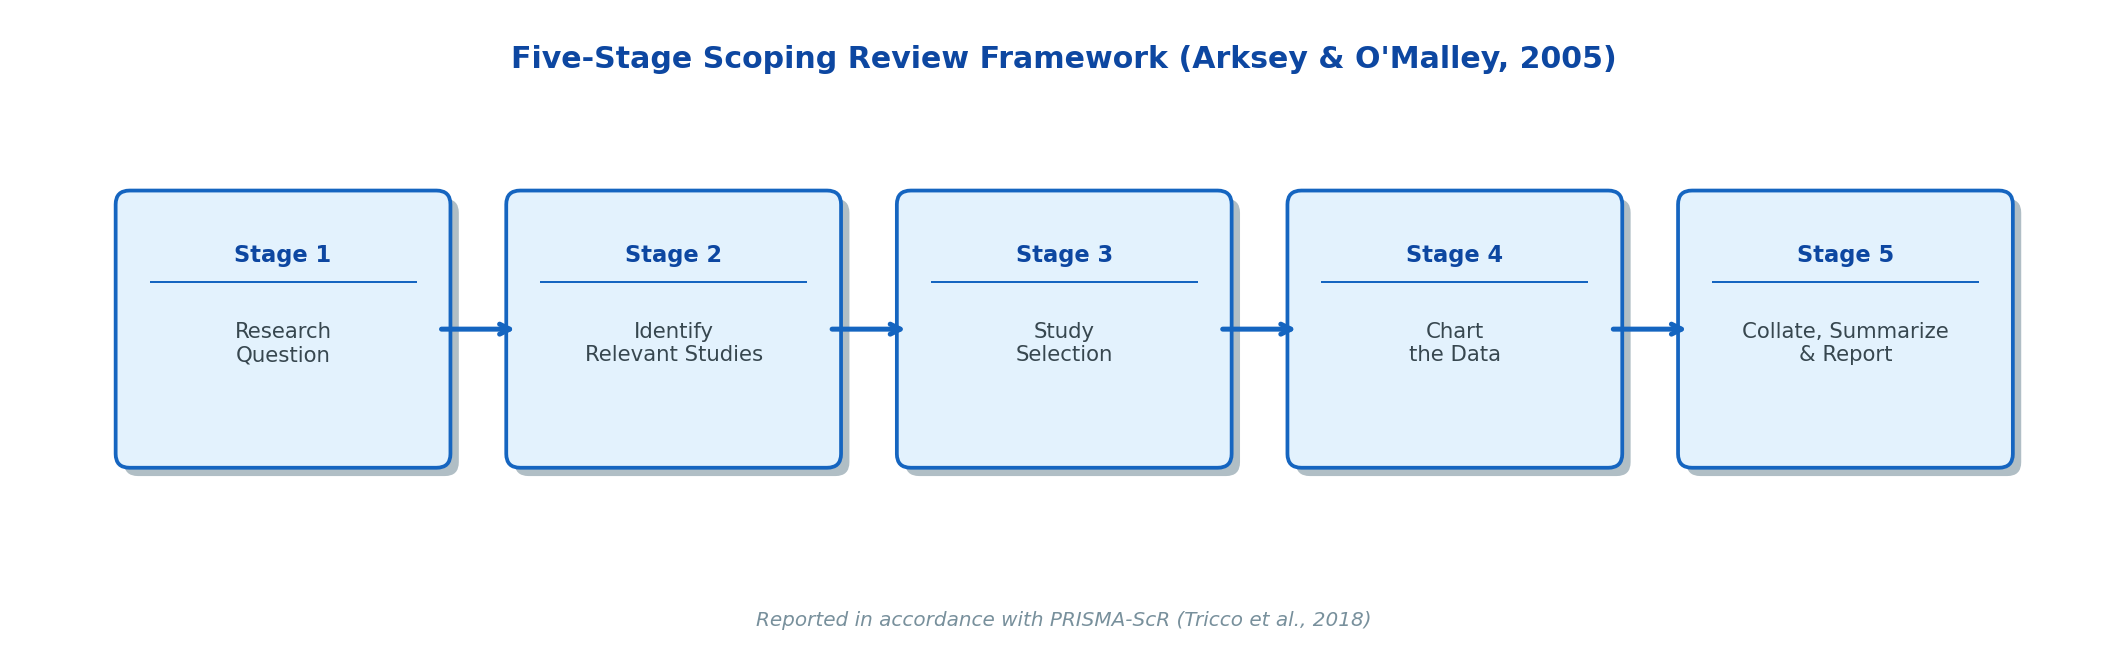
\includegraphics[width=\textwidth]{fig1_scoping_review_stages}
  \caption{Five-stage scoping review framework (Arksey \&
           O'Malley, 2005~\cite{b6}), applied in this study and
           reported in accordance with PRISMA-ScR
           (Tricco et al., 2018~\cite{b11}).}
  \label{fig:stages}
\end{figure*}


\subsection{PCC Framework and Operational Definitions}

Munn et al.~\cite{b7} recommend the Population-Concept-Context (PCC)
framework rather than PICO for scoping reviews, because the research
questions do not require an intervention component or an
experimentally measurable outcome. Table~\ref{tab:pcc} defines the
PCC elements in the present study.

\begin{table}[t]
  \caption{PCC Framework Definitions (Munn et al., 2018~\cite{b7})}
  \label{tab:pcc}
  \renewcommand{\arraystretch}{1.35}
  \begin{tabular}{@{} L{1.8cm} L{5.8cm} @{}}
    \toprule
    \textbf{Element} & \textbf{Definition in This Study} \\
    \midrule
    \textbf{Population}
      & Higher education institutions and their stakeholders:
        learners, instructors, and platform administrators \\[4pt]
    \textbf{Concept}
      & Frameworks and evaluation models designed for digital language
        learning platforms, including CALL, MALL, EdTech tools, and
        learning management systems \\[4pt]
    \textbf{Context}
      & Institutional adoption, quality assurance, and
        decision-making processes in higher education \\
    \bottomrule
  \end{tabular}
\end{table}

For the purposes of this review, an ``evaluation framework'' is a
conceptual instrument designed to assess the quality of a digital
platform from the perspective of system quality, content quality, or
institutional service. Teacher competency frameworks such as TPACK
are excluded because they assess teacher knowledge rather than
platform quality. Technology adoption models such as UTAUT are
included conditionally, provided their constructs have been adapted
as platform quality evaluation dimensions in the literature rather
than used solely as user acceptance predictors.


\subsection{Search Protocol}

The following databases were searched: Scopus (primary), Web of
Science, ERIC, and IEEE Xplore. The search period spans 2001 to
2025, beginning from Chapelle~\cite{b3} as the first landmark CALL
evaluation framework. Two search strings were applied in combination.

\noindent\textbf{String A (core):}
\begin{quote}
\small
(\textit{``evaluation framework''} OR \textit{``assessment model''} OR
\textit{``quality framework''} OR \textit{``evaluation criteria''})
AND
(\textit{``educational technology''} OR \textit{``e-learning''} OR
\textit{``CALL''} OR \textit{``MALL''} OR
\textit{``language learning platform''} OR \textit{``EdTech''} OR
\textit{``LMS''})
AND
(\textit{``higher education''} OR \textit{``university''} OR
\textit{``tertiary''})
\end{quote}

\noindent\textbf{String B (language-specific):}
\begin{quote}
\small
(\textit{``CALL evaluation''} OR \textit{``MALL evaluation''} OR
\textit{``language app evaluation''} OR
\textit{``test preparation platform''} OR \textit{``IELTS platform''} OR
\textit{``TOEFL platform''})
AND
(\textit{``framework''} OR \textit{``model''} OR \textit{``criteria''})
\end{quote}


\subsection{Inclusion and Exclusion Criteria}

Table~\ref{tab:criteria} specifies the criteria applied during
title-and-abstract screening and full-text review.

\begin{table*}[t]
  \caption{Inclusion and Exclusion Criteria}
  \label{tab:criteria}
  \renewcommand{\arraystretch}{1.3}
  \begin{tabular}{@{} L{2.2cm} L{6.5cm} L{6.5cm} @{}}
    \toprule
    \textbf{Criterion} & \textbf{Inclusion} & \textbf{Exclusion} \\
    \midrule
    Source type
      & Journal articles, book chapters, conference proceedings
        (peer-reviewed)
      & Grey literature, white papers, blogs, institutional reports \\
    Focus
      & Papers that present, propose, or critique an EdTech or CALL
        evaluation framework or model
      & Empirical studies that use a framework without developing it \\
    Context
      & Higher education; language learning; CALL, MALL, EdTech, LMS
      & K-12 contexts only; corporate training; non-educational
        platforms \\
    Language
      & English
      & Non-English \\
    Index
      & Scopus-indexed, WoS-indexed, ERIC, IEEE Xplore
      & Non-indexed journals; predatory journals (Beall's List or
        Cabells Blacklist) \\
    \bottomrule
  \end{tabular}
\end{table*}


\subsection{Theoretical Foundations of Analytical Dimensions}

The five analytical dimensions used in the coverage matrix were
derived from two complementary theoretical sources rather than
constructed ad hoc.

The first source is the DeLone and McLean IS Success
Model~\cite{b10}, which specifies three system-level quality
constructs: System Quality, Information Quality, and Service Quality.
These map directly to the technology, pedagogical, and institutional
dimensions of platform evaluation (D1, D2, and D3, respectively).
The model serves as a deductive meta-theory in this review, not as
an evaluated object. Including it in the corpus would create circular
reasoning, as the analytical dimensions would be derived from the
very framework under evaluation. It is therefore explicitly excluded
from the corpus (see Table~\ref{tab:corpus}).

The second source is language assessment theory, specifically
Bachman and Palmer~\cite{b12} and Chapelle~\cite{b3}. Authentic
assessment frameworks and SLA-based criteria require explicit
operationalization of high-stakes test metrics, which justifies D4
as a domain-specific dimension beyond the scope of general IS quality
theory. D6, the multi-stakeholder dimension, is derived from
Scheffel et al.~\cite{b9}, who identify multi-stakeholder perspective
as a distinct quality indicator for learning analytics tools in
higher education.

Table~\ref{tab:dimensions} defines all six analytical codes. D5 is
assessed as a separate framework rigor indicator rather than a
coverage dimension. Conflating framework meta-quality (D5) with
object-level coverage (D1--D4, D6) would produce non-equivalent
measurement categories.

\begin{table*}[t]
  \caption{Analytical Dimensions and Coding Definitions}
  \label{tab:dimensions}
  \renewcommand{\arraystretch}{1.35}
  \begin{tabular}{@{} C{0.6cm} L{2.5cm} L{5.0cm} L{4.8cm} @{}}
    \toprule
    \textbf{Code} & \textbf{Dimension}
      & \textbf{Operational Definition for Coding}
      & \textbf{Theoretical Source} \\
    \midrule
    D1 & Technology Architecture
      & Framework covers technical system quality: stability,
        adaptivity, accessibility, interface
      & DeLone \& McLean (2003)~\cite{b10}: System Quality \\
    D2 & Pedagogy Effectiveness
      & Framework covers content and instructional design: curriculum
        alignment, feedback, cognitive load, skill coverage
      & DeLone \& McLean (2003)~\cite{b10}: Information Quality \\
    D3 & Institutional Governance
      & Framework covers institutional aspects: analytics, monitoring,
        decision-support, data interoperability
      & DeLone \& McLean (2003)~\cite{b10}: Service Quality \\
    D4 & High-Stakes Test Specificity
      & Framework explicitly operationalizes metrics for high-stakes
        testing contexts (IELTS, TOEFL, CEFR alignment)
      & Bachman \& Palmer (2010)~\cite{b12}; Chapelle
        (2001)~\cite{b3} \\
    D6 & Multi-Stakeholder Perspective
      & Framework accommodates more than one stakeholder type
        (learner, instructor, and administrator)
      & Scheffel et al. (2014)~\cite{b9} \\
    \midrule
    D5\textsuperscript{\dag} & Framework Rigor
      & Presence of systematic operational definitions rather than
        reflective checklists
      & Munn et al. (2018)~\cite{b7} [meta-level indicator only;
        not counted in coverage score] \\
    \bottomrule
    \multicolumn{4}{@{}l@{}}{\footnotesize \textsuperscript{\dag}D5
      assesses the framework's own methodological quality, not a
      platform quality dimension; it is scored in a separate column.}
  \end{tabular}
\end{table*}

\begin{figure*}[t]
  \centering
  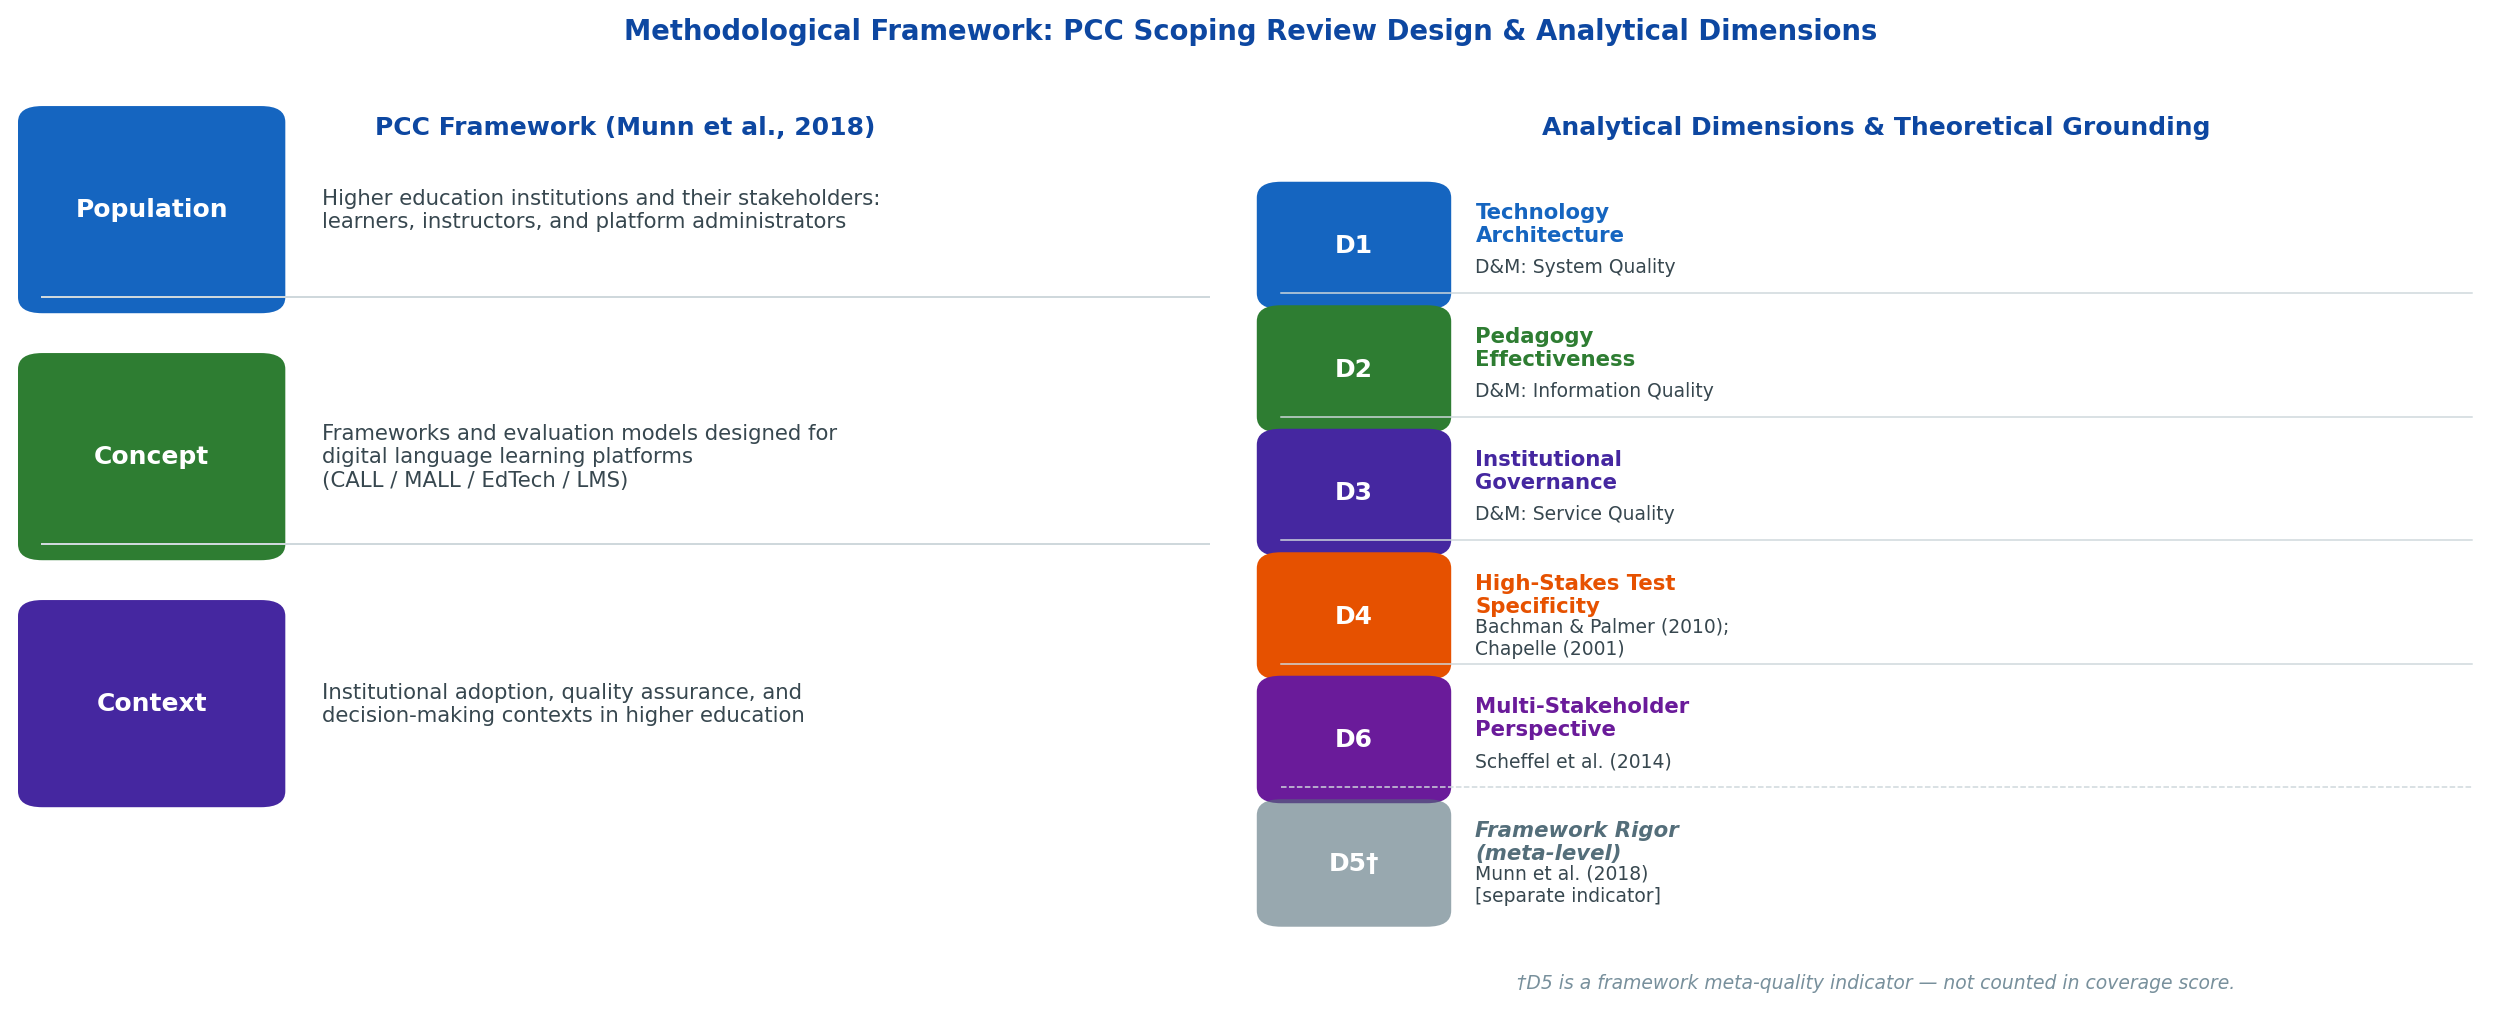
\includegraphics[width=\textwidth]{fig6_pcc_and_dimensions}
  \caption{PCC framework elements and analytical dimension grounding.
           Left panel: Population-Concept-Context definitions per
           Munn et al.~\cite{b7}. Right panel: all six analytical
           codes (D1--D4, D6, and D5\textsuperscript{\dag}) with
           their theoretical sources.}
  \label{fig:pcc_dims}
\end{figure*}


\subsection{Data Charting and Coding Scheme}

Each included framework was analyzed through an extraction form that
coded five analytical dimensions (D1, D2, D3, D4, D6), with D5
scored separately. Three coverage levels were defined: full coverage
(scored 1.0), partial coverage (0.5), and no coverage (0.0). A
dimension receives \fullcov{} (full) when it is explicitly defined
and operationalized in the framework; \partcov{} (partial) when it
is mentioned but not operationally defined or only implicit; and
\nocov{} (absent) when it is entirely missing.

The overall coverage score for each framework is:
\begin{equation}
  \text{Coverage Score} =
    \sum_{i \in \{D1,\, D2,\, D3,\, D4,\, D6\}} s_i,
  \quad s_i \in \{0,\; 0.5,\; 1.0\}
  \label{eq:score}
\end{equation}
with a maximum achievable score of 5.0.


\subsection{Inter-Rater Reliability}

A second independent coder scored a minimum of 20\,\% of all
included frameworks. Agreement was measured with Cohen's Kappa
($\kappa$), with a minimum acceptable threshold of $\kappa \geq
0.80$. Disagreements were resolved through consensus discussion;
unresolved cases were referred to a third arbitrator. Kappa values
per dimension are reported alongside the coverage matrix in
Section~\ref{sec:results}.


\subsection{Pre-Registration}

This study's protocol was registered on the Open Science Framework
(OSF) prior to the database search phase. Because the literature
search and coverage matrix data are shared with a companion study on
integrated framework construction, the nature of this shared data
collection was disclosed in the OSF registration and will be
disclosed to the editor in the cover letter at submission.


% ============================================================
\section{Results}
\label{sec:results}
% ============================================================

\subsection{Framework Corpus}

A total of 12 frameworks were identified for inclusion following the
database search and screening procedure (PRISMA-ScR flow diagram
[to be inserted in the final version after Phase~2 execution]).
Table~\ref{tab:corpus} presents the complete corpus. Frameworks
originate from four disciplines: Applied Linguistics (F1--F5), IS
(F6, F7, F10, F11), Learning Analytics (F8, F9), and a recent
IS-linguistics hybrid category (F12). Publication dates range from
2001 to 2025, spanning the full search window.

Two frameworks were explicitly excluded from the corpus and treated as
theoretical sources instead. DeLone and McLean~\cite{b10} function as
a deductive meta-theory used to derive D1, D2, and D3; their inclusion
would create circular reasoning in the coverage analysis. The TPACK
model assesses teacher technological-pedagogical-content knowledge
rather than platform quality; it therefore falls outside the
operational definition of an evaluation framework adopted in this
study.

\begin{table*}[t]
  \caption{Framework Corpus: 12 Evaluation Frameworks Included in the Analysis}
  \label{tab:corpus}
  \renewcommand{\arraystretch}{1.3}
  \begin{tabular}{@{} C{0.5cm} L{4.2cm} L{2.8cm} L{3.0cm} C{1.0cm} @{}}
    \toprule
    \textbf{\#} & \textbf{Framework} & \textbf{Discipline}
      & \textbf{Context} & \textbf{Year} \\
    \midrule
    F1  & Chapelle --- SLA-based 6 Criteria~\cite{b3}
        & Applied Linguistics & CALL                     & 2001 \\
    F2  & Hubbard --- Process-oriented Evaluation~\cite{b8}
        & Applied Linguistics & CALL courseware           & 2011 \\
    F3  & Leakey --- Integrated 12 Criteria~\cite{b4}
        & Applied Linguistics & CALL                     & 2011 \\
    F4  & Colpaert --- RBRO Model
        & Instructional Design & CALL                    & 2004 \\
    F5  & Rosell-Aguilar --- MALL Taxonomy~\cite{b1}
        & Applied Linguistics & MALL apps                & 2017 \\
    F6  & Almaiah et al. --- Delphi 6-Dimension~\cite{b5}
        & Information Systems & E-learning               & 2021 \\
    F7  & Al-Fraihat et al. --- E-learning Success~\cite{b2}
        & Information Systems & E-learning / LMS         & 2020 \\
    F8  & Scheffel et al. --- EFLA~\cite{b9}
        & Learning Analytics  & HE learning tools        & 2014 \\
    F9  & Park \& Jo --- LAD (Kirkpatrick-based)~\cite{b13}
        & Learning Analytics  & HE dashboard             & 2019 \\
    F10 & Venkatesh et al. --- UTAUT
        & Information Systems & Technology adoption      & 2003 \\
    F11 & Kampa et al. --- TRAM
        & Information Systems & Language EdTech          & 2024 \\
    F12 & Essafi --- MLLA 3-Aspect
        & Applied Linguistics & MALL                     & 2025 \\
    \bottomrule
    \multicolumn{5}{@{}l@{}}{\footnotesize
      Excluded from corpus (treated as analytical sources):
      DeLone \& McLean~\cite{b10} (deductive meta-theory for D1--D3;
      inclusion would create circular reasoning) and TPACK (teacher
      knowledge model, not a platform quality evaluation instrument).}
  \end{tabular}
\end{table*}


\subsection{Coverage Matrix}

Table~\ref{tab:matrix} presents the complete dimensional coverage
matrix; Fig.~\ref{fig:heatmap} provides the corresponding visual
heatmap with coverage scores plotted alongside each framework.
Fig.~\ref{fig:scores} shows the ranked distribution of scores across
the corpus. Three findings emerge from the matrix.

\textit{Finding 1 (Maximum coverage cap):} No single framework
exceeds a coverage score of 2.5/5.0 (50\,\%). The two
highest-scoring frameworks, F6 (Almaiah et al., 2021~\cite{b5}) and
F7 (Al-Fraihat et al., 2020~\cite{b2}), both reach this maximum.

\textit{Finding 2 (Dimension-specific ceiling):} D4 (High-Stakes Test
Specificity) and D6 (Multi-Stakeholder Perspective) are the only two
dimensions that achieve no full coverage in any framework; both
reach a maximum of \partcov{} (partial). D3 (Institutional
Governance) is fully covered only in F8 and F9, both learning
analytics tools designed for general higher education contexts rather
than for language platform evaluation.

\textit{Finding 3 (Rigor deficit):} With respect to D5 (Framework
Rigor), 7 of the 12 frameworks provide partial operational
definitions, and 5 rely on reflective checklists without systematic
measurement operationalization. No framework in this corpus achieves
full D5 rigor.

\begin{table*}[t]
  \caption{Dimensional Coverage Matrix
    ($\fullcov{}$ Full~=~1.0;\;
     $\partcov{}$ Partial~=~0.5;\;
     $\nocov{}$ Absent~=~0.0.\;
     D5 Rigor is a separate indicator and is not counted in the score.)}
  \label{tab:matrix}
  \renewcommand{\arraystretch}{1.35}
  \setlength{\tabcolsep}{5pt}
  \begin{tabular*}{\textwidth}{@{\extracolsep{\fill}}
      L{3.4cm}
      C{1.0cm} C{1.0cm} C{1.0cm} C{1.6cm} C{1.7cm}
      C{1.3cm}
      C{1.1cm} @{}}
    \toprule
    \textbf{Framework}
      & \textbf{D1\newline TECH}
      & \textbf{D2\newline PED}
      & \textbf{D3\newline INST}
      & \textbf{D4\newline High-Stakes}
      & \textbf{D6\newline Multi-Stakeholder}
      & \textbf{Score\newline /5.0}
      & \textbf{D5\newline Rigor\textsuperscript{\dag}} \\
    \midrule
    F1\; Chapelle (2001)       & \nocov  & \fullcov & \nocov  & \partcov & \nocov  & 1.5 & \partcov \\
    F2\; Hubbard (2011)        & \nocov  & \fullcov & \nocov  & \nocov   & \nocov  & 1.0 & \partcov \\
    F3\; Leakey (2011)         & \partcov& \fullcov & \nocov  & \nocov   & \nocov  & 1.5 & \partcov \\
    F4\; Colpaert (2004)       & \nocov  & \fullcov & \nocov  & \nocov   & \nocov  & 1.0 & \partcov \\
    F5\; Rosell-Aguilar (2017) & \partcov& \partcov & \nocov  & \nocov   & \nocov  & 1.0 & \nocov   \\
    F6\; Almaiah et al. (2021) & \fullcov& \partcov & \partcov& \nocov   & \partcov& 2.5 & \nocov   \\
    F7\; Al-Fraihat et al. (2020)
                               & \fullcov& \partcov & \partcov& \nocov   & \partcov& 2.5 & \partcov \\
    F8\; Scheffel/EFLA (2014)  & \nocov  & \nocov   & \fullcov& \nocov   & \partcov& 1.5 & \partcov \\
    F9\; Park \& Jo (2019)     & \nocov  & \nocov   & \fullcov& \nocov   & \partcov& 1.5 & \partcov \\
    F10 UTAUT/Venkatesh (2003) & \partcov& \nocov   & \nocov  & \nocov   & \nocov  & 0.5 & \nocov   \\
    F11 TRAM/Kampa (2024)      & \partcov& \partcov & \nocov  & \nocov   & \nocov  & 1.0 & \nocov   \\
    F12 Essafi/MLLA (2025)     & \partcov& \fullcov & \nocov  & \partcov & \nocov  & 2.0 & \nocov   \\
    \midrule
    \textbf{Max (any single)}
      & \fullcov & \fullcov & \fullcov & \partcov & \partcov
      & \textbf{2.5} & \partcov \\
    \bottomrule
    \multicolumn{8}{@{}l@{}}{\footnotesize
      \textsuperscript{\dag}D5 Rigor: \partcov\ = partial operational
      definitions; \nocov\ = reflective checklist only;
      \fullcov\ = full operationalization (achieved by none in this corpus).}
  \end{tabular*}
\end{table*}

\begin{figure*}[t]
  \centering
  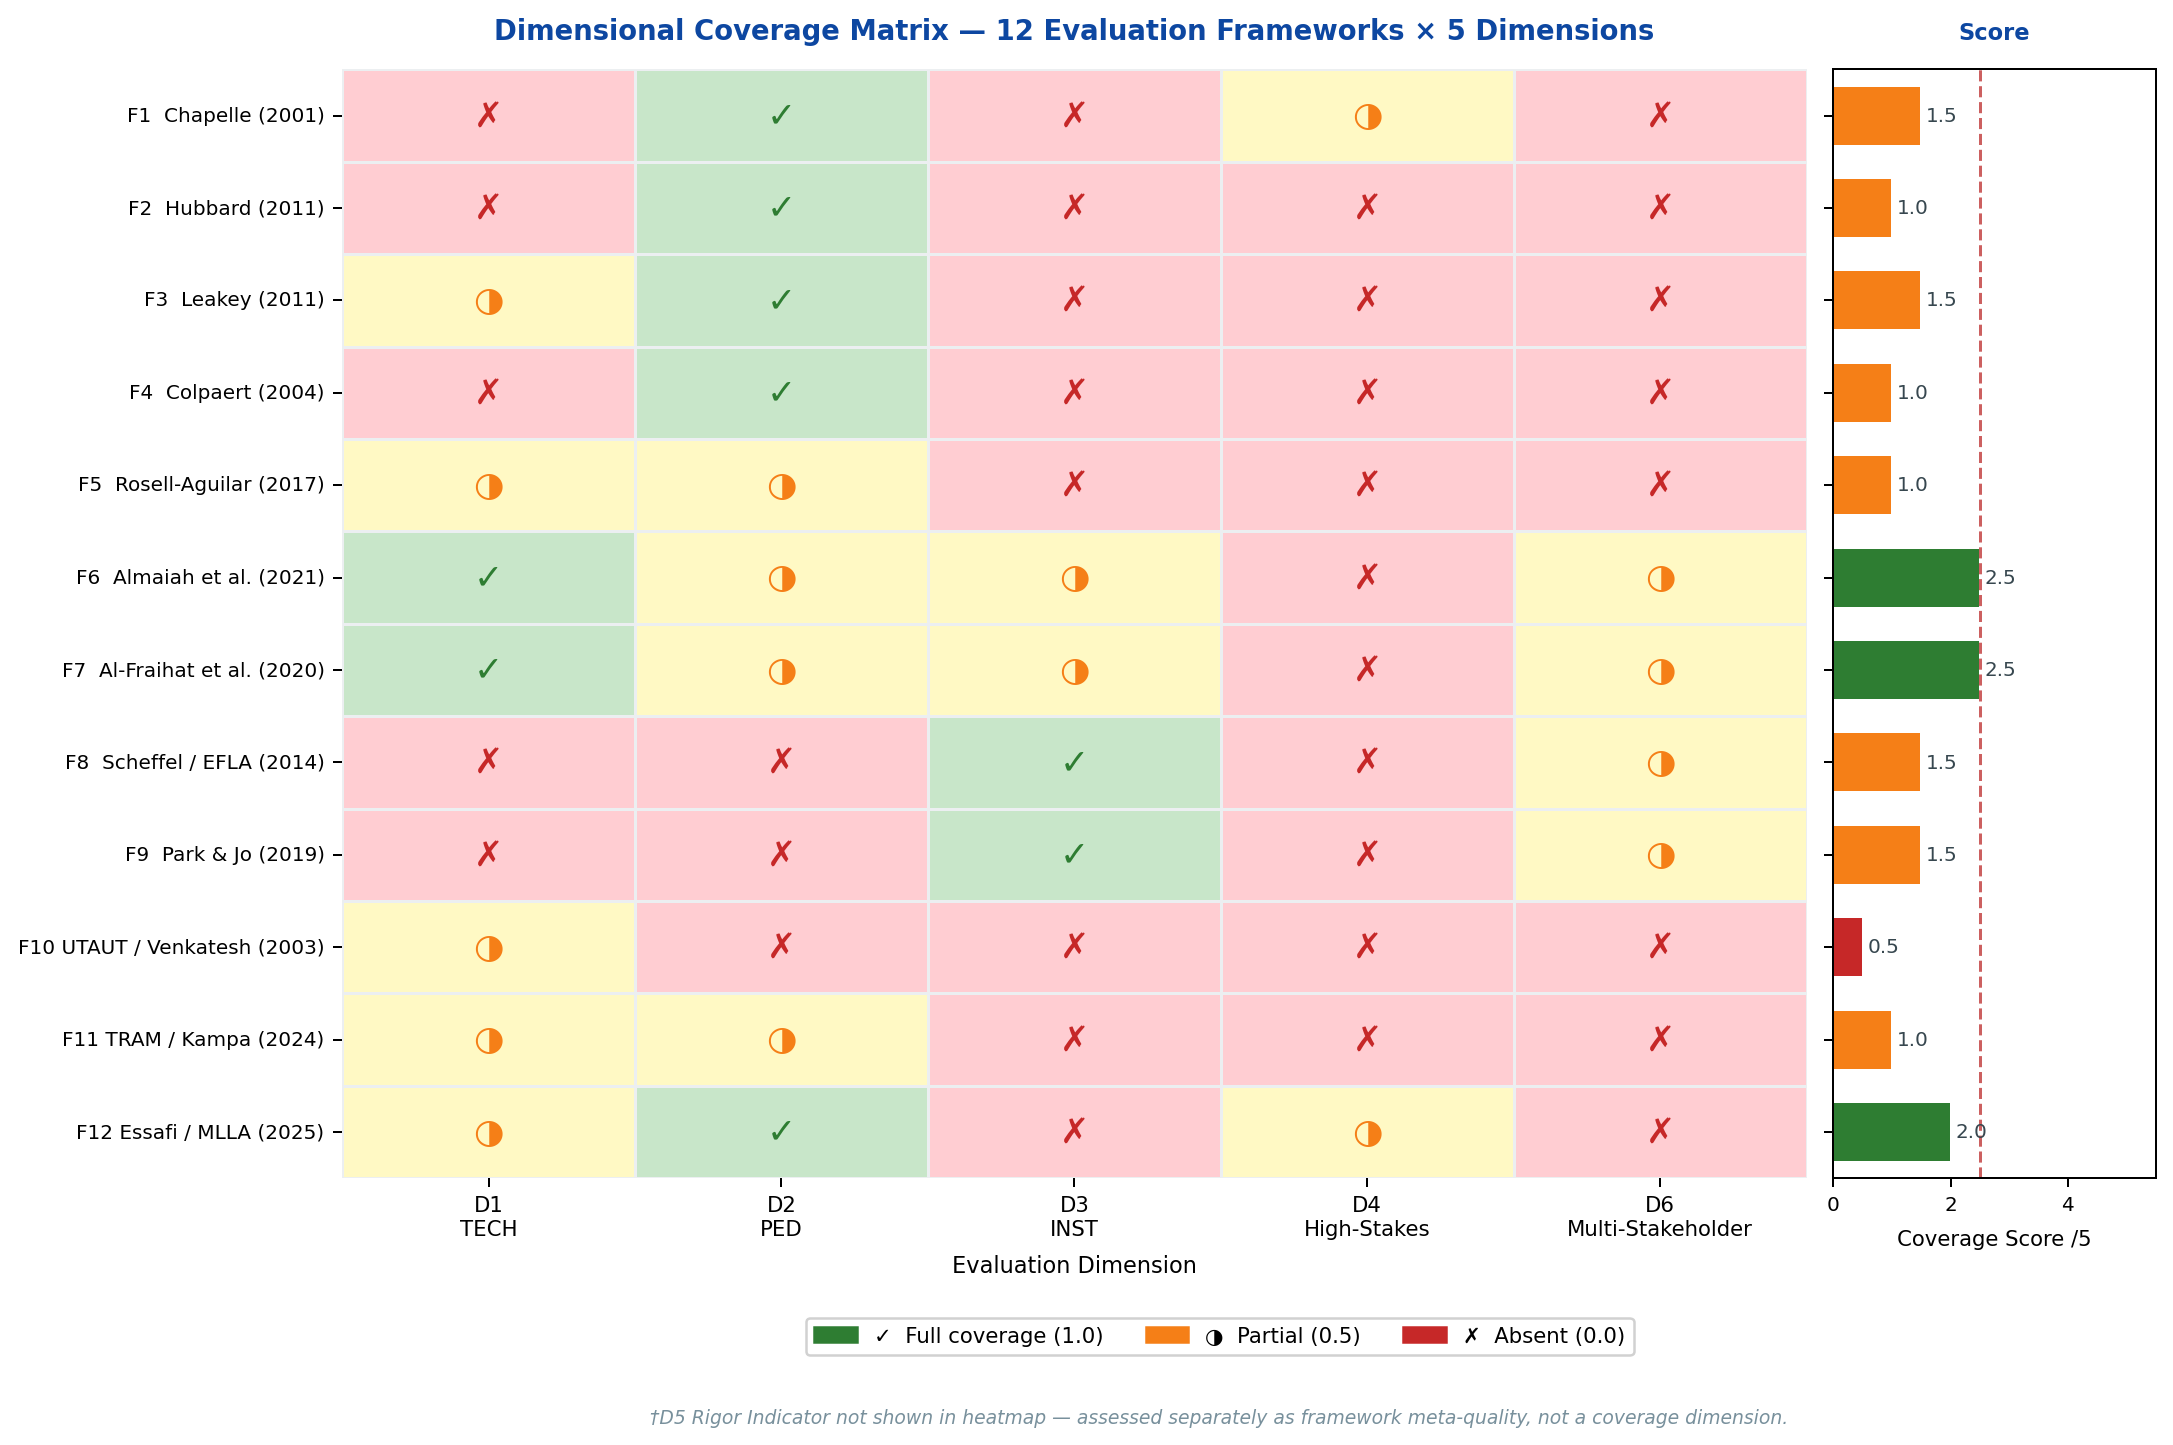
\includegraphics[width=\textwidth]{fig2_coverage_matrix_heatmap}
  \caption{Coverage matrix heatmap for 12 evaluation frameworks across
           five object-level dimensions. Green ($\fullcov{}$) = full
           coverage (1.0); amber ($\partcov{}$) = partial (0.5); red
           ($\nocov{}$) = absent (0.0). The right panel shows coverage
           scores ranked from highest (2.5) to lowest (0.5). No framework
           exceeds 50\,\% of the maximum possible coverage.}
  \label{fig:heatmap}
\end{figure*}

\begin{figure}[t]
  \centering
  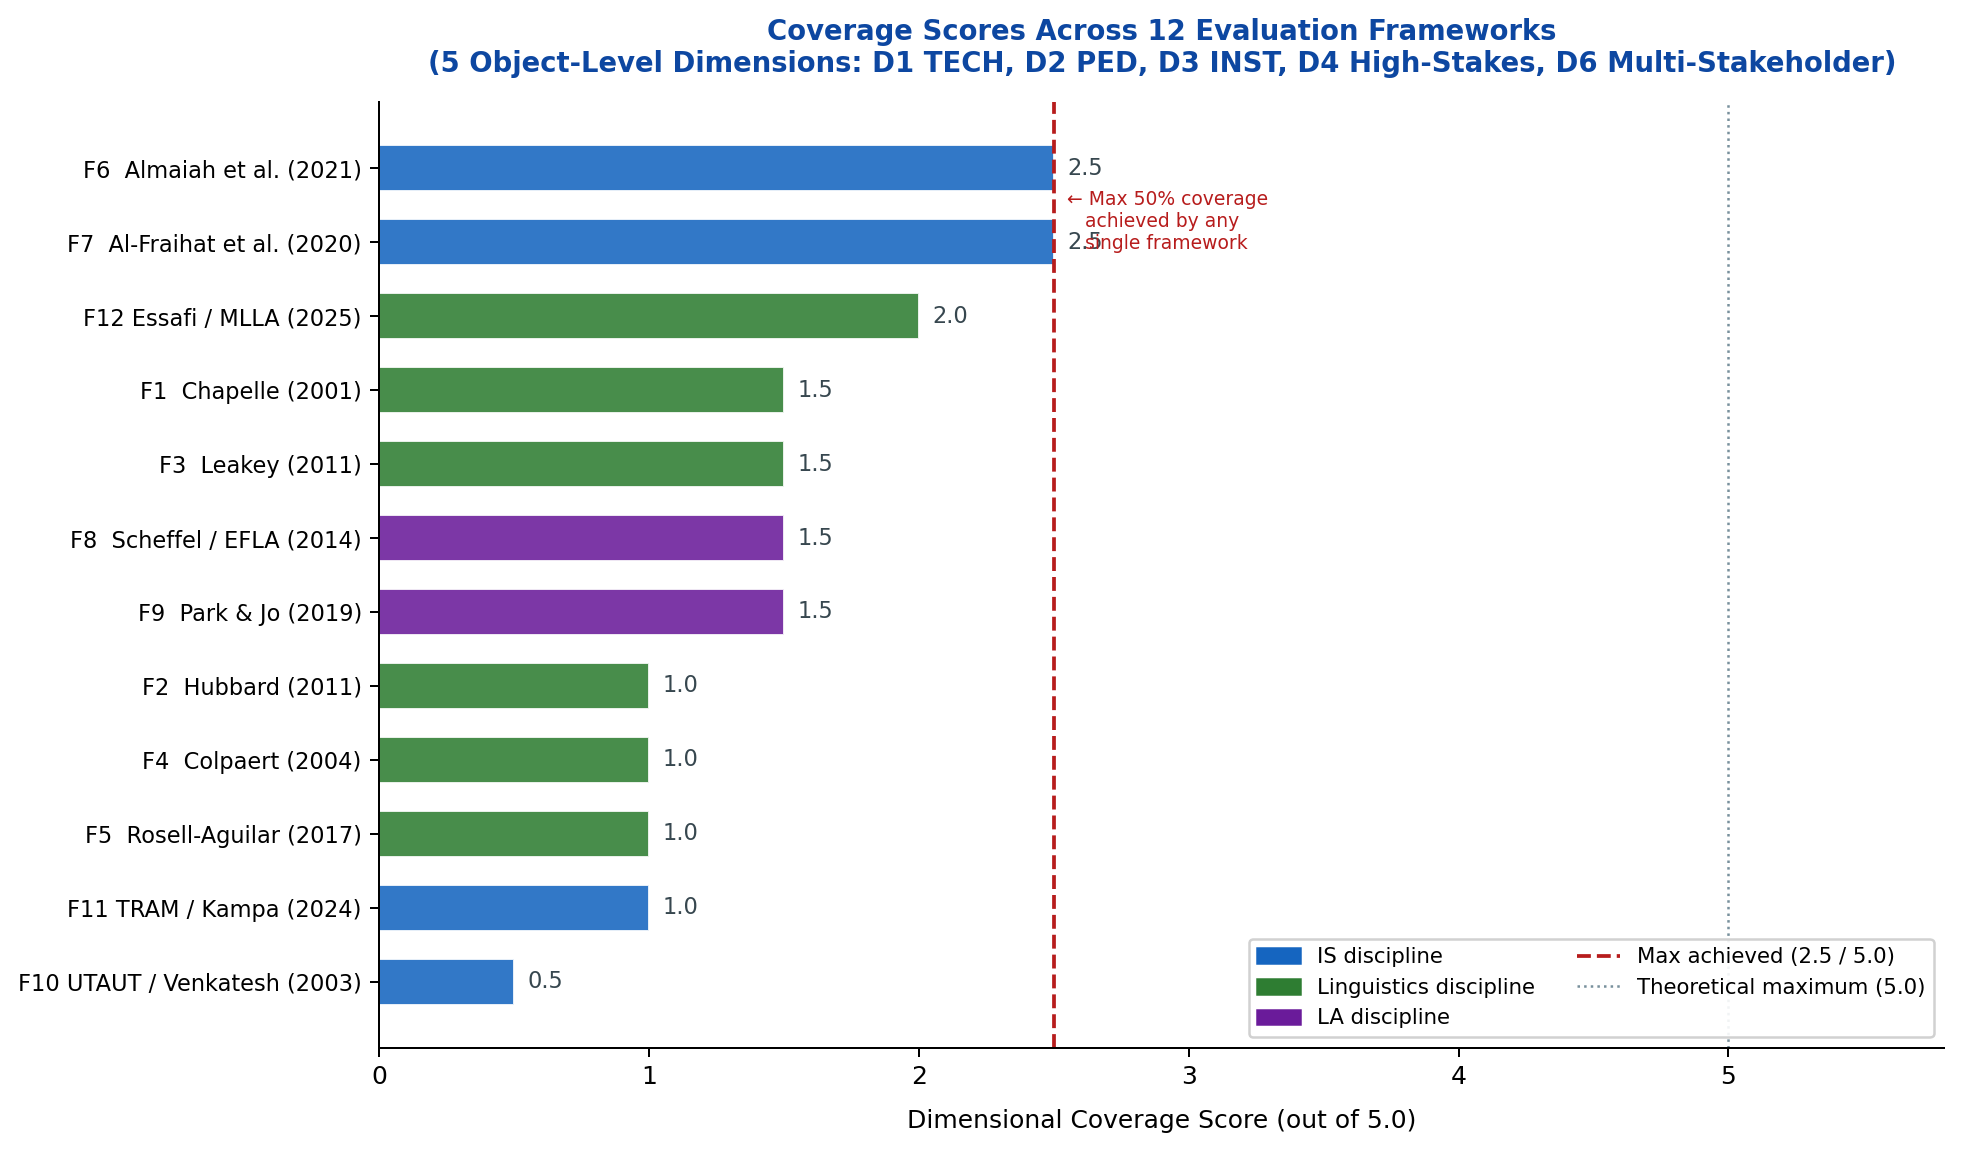
\includegraphics[width=\columnwidth]{fig3_coverage_scores_ranked}
  \caption{Coverage scores across 12 evaluation frameworks, ranked from
           highest to lowest. Bar colour indicates discipline of origin:
           blue = IS; green = Applied Linguistics; purple = Learning
           Analytics. The dashed red line marks the maximum observed
           score of 2.5/5.0.}
  \label{fig:scores}
\end{figure}


\subsection{Dimensional Gap Analysis}

The coverage matrix reveals four systematic gaps, illustrated in
Fig.~\ref{fig:gaps}.

\textit{Gap 1 (Contextual Specificity):} D4 reaches partial coverage
in only two frameworks (F1 and F12) and is entirely absent from the
remaining ten. No framework provides a fully operationalized set of
high-stakes test metrics. This finding reflects the disciplinary
origins of most CALL frameworks: SLA theory specifies what effective
language learning looks like but does not translate that specification
into platform-deliverable test preparation metrics.

\textit{Gap 2 (Disciplinary Silos):} CALL frameworks (F1--F5) cover
D2 consistently but score 0.0 on D1 (with the exception of partial
coverage in F3 and F5) and 0.0 on D3 uniformly. IS frameworks (F6,
F7) cover D1 and partially approach D3 but operationalize D2 as
generic information quality rather than language-specific pedagogical
effectiveness. Neither tradition crosses into the other's conceptual
domain.

\textit{Gap 3 (Institutional Blindspot):} D3 is fully covered only in
F8 and F9, both learning analytics dashboards. All five CALL and MALL
frameworks (F1--F5) score 0.0 on D3. This pattern is consistent with
the disciplinary scope of CALL evaluation, which concentrates on the
learning interaction rather than on institutional management and
decision-support.

\textit{Gap 4 (Single-Stakeholder Bias):} D6 reaches partial coverage
in F6, F7, F8, and F9, and is entirely absent from all remaining
frameworks. No framework fully operationalizes evaluation from the
simultaneous perspectives of learners, instructors, and platform
administrators.

A separate rigor finding complements the four coverage gaps: 5 of the
12 frameworks amount to reflective checklists without adequate
operational definitions (D5 = \nocov). Adoption decisions that rely
on these five frameworks cannot be audited or systematically
replicated.

\begin{figure*}[t]
  \centering
  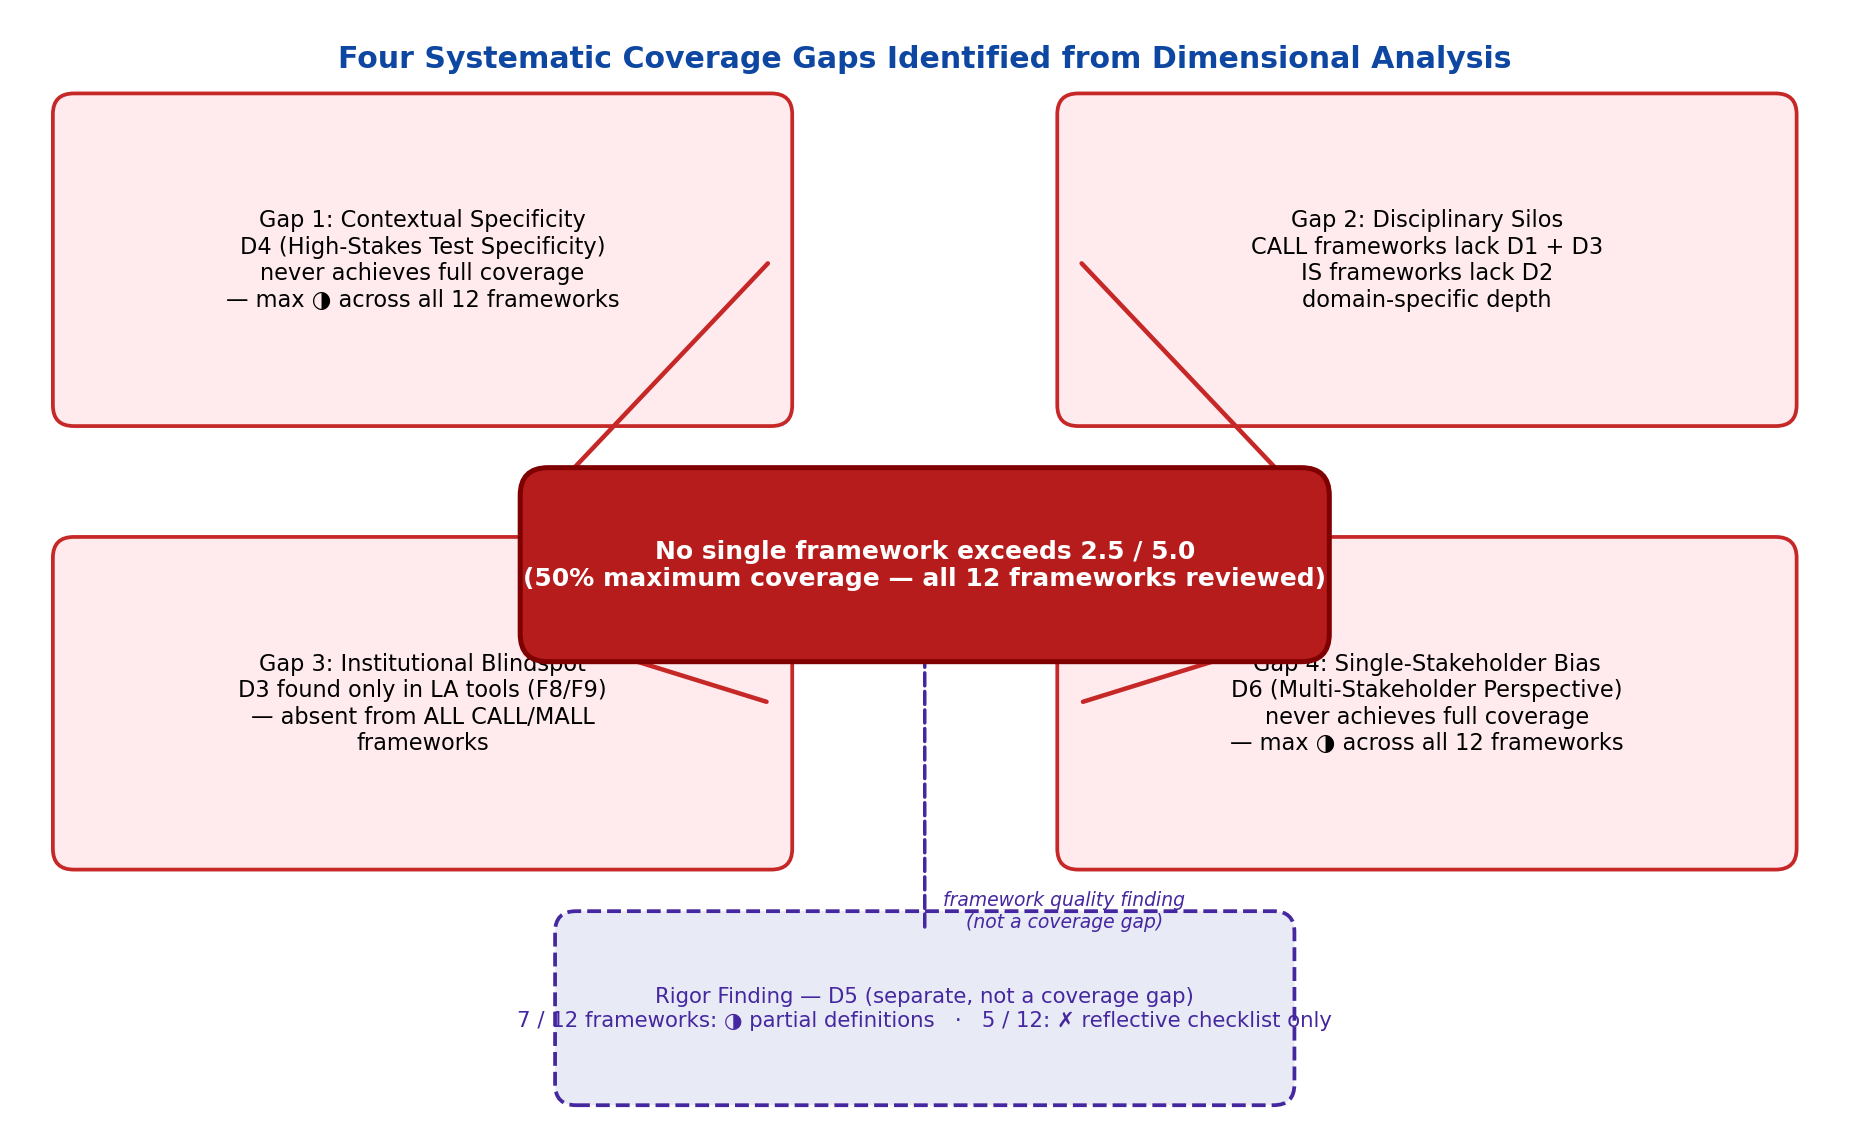
\includegraphics[width=\textwidth]{fig4_coverage_gaps_diagram}
  \caption{Four systematic coverage gaps identified from the dimensional
           analysis. Each gap box (red) converges on the central finding
           that no framework exceeds 2.5/5.0. The dashed purple box
           (lower centre) shows the D5 rigor finding, which is a
           framework meta-quality observation rather than a coverage gap
           and is therefore not counted in the coverage score.}
  \label{fig:gaps}
\end{figure*}


% ============================================================
\section{Discussion}
\label{sec:discussion}
% ============================================================

\subsection{Theoretical Implications}

The absence of any framework with full dimensional coverage is not
coincidental; it reflects structural disciplinary fragmentation in the
EdTech evaluation literature. Applied Linguistics researchers build
evaluation outward from SLA theory, so technical and institutional
dimensions fall outside their conceptual scope by design. IS
researchers build inward from system quality models, so
pedagogical domain-specificity, particularly the distinctions required
for high-stakes test preparation, is not treated as a system quality
concern. These are not individual oversights; they are the predictable
consequences of discipline-bounded research traditions.

This analysis indicates that closing the gap requires more than
extending existing frameworks. It requires a bridging ontology that
explicitly integrates IS meta-theory, language assessment theory, and
institutional governance into a single measurement architecture.
The DeLone and McLean model~\cite{b10}, which integrates system,
information, and service quality under a unified IS success construct,
provides the ontological structure most suited to this role. An
integrated framework built on DeLone and McLean as the meta-theoretical
foundation would, in principle, accommodate D1, D2, and D3 within a
single coherent architecture and could be extended with D4 and D6 as
domain-specific supplements.

Prior studies have shown that IS meta-theories provide productive
organizing structures for technology evaluation across domains. The
DeLone and McLean update published in 2003~\cite{b10} explicitly
extended the original model to encompass service quality and
net-benefit measures, anticipating the multi-level assessment problem
documented in this review. The coverage matrix provides, for the first
time, the empirical evidence needed to justify applying this extension
to the language learning platform domain.

\subsection{Practical Implications}

For higher education administrators, the results have direct operational
consequences: no single framework is adequate for comprehensive adoption
decision-making. The highest-scoring frameworks, F6 and F7 both at
2.5/5, still fail to cover D4 entirely and cover D6 only partially.
Administrators who rely on either framework alone will systematically
underweight test-specificity criteria and will collect stakeholder
perspectives from only a subset of relevant actors.

The coverage matrix also enables evidence-based strategic combinations.
Administrators concerned with technical alignment and pedagogical
completeness may combine F7 (strongest on D1 and D3 approach, IS
discipline) with F1 Chapelle (strongest on D2 and partial D4, Applied
Linguistics). Together, this combination covers D1, D2, D3, and
partial D4. D6 remains a collective blindspot, inadequately covered by
any combination in the present corpus. The matrix therefore serves not
only as a gap catalogue but as an evidence-based decision instrument
for current practice while the field awaits a comprehensive framework.

The D5 findings carry separate implications for evidence-based
technology governance. The five frameworks that score \nocov{} on D5
provide no systematic measurement operationalization. Institutions
that implement formal technology governance processes need to attend
not only to what a framework covers but also to how operationalized
its dimensions are. Unreplicable checklist-based assessments cannot
accumulate institutional knowledge across adoption cycles.

\subsection{Limitations}

This review has four inherent limitations. First, although the
IRR procedure was implemented, residual subjectivity in dimensional
coding cannot be entirely eliminated; the reported $\kappa$ values
reflect agreement achieved but do not guarantee objective
classification. Second, restricting the search to English-language
literature may exclude frameworks from non-Anglophone research
traditions, particularly those from East Asia and Latin America.
Third, frameworks published in 2024 and 2025 may not be fully indexed
in all searched databases at the time of retrieval, which could
underrepresent the most recent methodological developments. Fourth,
the operational definitions of the five analytical dimensions represent
the interpretations of the research team; researchers from different
disciplines may operationalize these dimensions differently, which
would alter some coding decisions.


% ============================================================
\section{Conclusion}
\label{sec:conclusion}
% ============================================================

This scoping review systematically mapped 12 evaluation frameworks for
digital language learning and EdTech platforms in higher education
against five object-level evaluation dimensions and one framework
rigor indicator. The three research questions are answered as follows.

\textit{RQ1:} The review identified 12 frameworks from four
disciplines: Applied Linguistics (CALL and MALL), IS, Learning
Analytics, and a recent IS-linguistics hybrid. No single discipline
provides comprehensive coverage. CALL produces the most frameworks but
is restricted to the pedagogical dimension; IS produces technically
more complete frameworks but lacks language and test domain
specificity.

\textit{RQ2:} D2 (Pedagogy Effectiveness) is the most consistently
covered dimension across the corpus. D4 (High-Stakes Test Specificity)
and D6 (Multi-Stakeholder Perspective) never achieve full coverage;
both reach a maximum of partial coverage. D3 (Institutional
Governance) is fully covered only in learning analytics tools not
designed as language platform evaluation instruments. Five of the
12 frameworks lack adequate operational definitions (D5), rendering
them unsuitable for systematic and reproducible assessment.

\textit{RQ3:} No framework simultaneously covers D1, D2, and D3
together with D4 and D6, even at partial levels. The maximum coverage
score observed across the entire corpus is 2.5/5.0 (50\,\%).

Three research directions follow from these results. First, a
framework that bridges IS and Applied Linguistics is needed, with the
DeLone and McLean model~\cite{b10} as the unifying meta-theoretical
foundation. Second, D4 (high-stakes test specificity) requires
operationalization; it is systematically absent from all existing
frameworks. Third, the institutional governance perspective (D3) needs
to be integrated into language platform evaluation instruments, drawing
on the data analytics capabilities already present in IS-oriented
tools.

The coverage matrix produced in this study provides the empirical
baseline needed to justify that programme of framework development.


% ============================================================
% References
% ============================================================
\begin{thebibliography}{00}

\bibitem{b1}
F. Rosell-Aguilar, ``State of the app: A taxonomy and framework for
evaluating language learning mobile applications,'' \textit{CALICO J.},
vol.~34, no.~2, pp.~243--258, 2017.

\bibitem{b2}
D. Al-Fraihat, M. Joy, R. Masa'deh, and J. Sinclair, ``Evaluating
e-learning systems success: An empirical study,'' \textit{Comput.
Hum. Behav.}, vol.~102, pp.~67--86, 2020. [Online]. Available:
\url{https://doi.org/10.1016/j.chb.2019.08.004}

\bibitem{b3}
C. A. Chapelle, \textit{Computer Applications in Second Language
Acquisition: Foundations for Teaching, Testing and Research}.
Cambridge, U.K.: Cambridge Univ. Press, 2001.

\bibitem{b4}
J. Leakey, \textit{Evaluating Computer-Assisted Language Learning:
An Integrated Approach to Effectiveness Research in CALL}. Bern,
Switzerland: Peter Lang, 2011.

\bibitem{b5}
M. A. Almaiah, A. Al-Khasawneh, and A. Althunibat, ``Exploring the
critical challenges and factors influencing the e-learning system usage
during COVID-19 pandemic,'' \textit{Educ. Inf. Technol.}, vol.~26,
no.~5, pp.~5261--5280, 2021. [Online]. Available:
\url{https://doi.org/10.1007/s10639-021-10523-y}

\bibitem{b6}
H. Arksey and L. O'Malley, ``Scoping studies: Towards a methodological
framework,'' \textit{Int. J. Soc. Res. Methodol.}, vol.~8, no.~1,
pp.~19--32, 2005. [Online]. Available:
\url{https://doi.org/10.1080/1364557032000119616}

\bibitem{b7}
Z. Munn, M. D. J. Peters, C. Stern, C. Tufanaru, A. McArthur, and
E. Aromataris, ``Systematic review or scoping review? Guidance for
authors when choosing between a systematic or scoping review
approach,'' \textit{Syst. Rev.}, vol.~7, no.~1, p.~143, 2018.
[Online]. Available: \url{https://doi.org/10.1186/s13643-018-0611-5}

\bibitem{b8}
P. Hubbard, ``Evaluation of courseware and websites,'' in \textit{Present
and Future Promises of CALL}, L. Ducate and N. Arnold, Eds. San Marcos,
TX: CALICO, 2011, pp.~407--440.

\bibitem{b9}
M. Scheffel, H. Drachsler, S. Stoyanov, and M. Specht, ``Quality
indicators for learning analytics,'' \textit{Educ. Technol. Soc.},
vol.~17, no.~4, pp.~117--132, 2014.

\bibitem{b10}
W. H. DeLone and E. R. McLean, ``The DeLone and McLean model of
information systems success: A ten-year update,'' \textit{J. Manage.
Inf. Syst.}, vol.~19, no.~4, pp.~9--30, 2003. [Online]. Available:
\url{https://doi.org/10.1080/07421222.2003.11045748}

\bibitem{b11}
A. C. Tricco et al., ``PRISMA extension for scoping reviews (PRISMA-ScR):
Checklist and explanation,'' \textit{Ann. Intern. Med.}, vol.~169,
no.~7, pp.~467--473, 2018. [Online]. Available:
\url{https://doi.org/10.7326/M18-0850}

\bibitem{b12}
L. F. Bachman and A. S. Palmer, \textit{Language Assessment in
Practice}. Oxford, U.K.: Oxford Univ. Press, 2010.

\bibitem{b13}
Y. Park and I.-H. Jo, ``Development of the learning analytics dashboard
to support students' learning performance,'' \textit{J. Comput. Assist.
Learn.}, vol.~35, no.~4, pp.~556--568, 2019. [Online]. Available:
\url{https://doi.org/10.1111/jcal.12354}

\bibitem{b14}
D. Levac, H. Colquhoun, and K. K. O'Brien, ``Scoping studies: Advancing
the methodology,'' \textit{Implement. Sci.}, vol.~5, no.~1, p.~69,
2010. [Online]. Available:
\url{https://doi.org/10.1186/1748-5908-5-69}

\end{thebibliography}

\end{document}
